% ===== SLIDE: Training Strategy & Datasets =====
\begin{frame}{Training Strategy \& Datasets}
    \begin{columns}[T]
    \column{0.48\textwidth}
        \begin{block}{Loss Functions}
            \small
            The network is trained end-to-end using a multi-task objective:
            \begin{enumerate}\setlength\itemsep{2pt}
                \item \textbf{Identity Loss (Cross-Entropy):} Ensures the extracted features are highly discriminative for the specific person ID.
                \item \textbf{Triplet Loss:} Pulls features of the same person closer together while pushing apart features of different people.
            \end{enumerate}
            \smallskip
        \end{block}

    \column{0.48\textwidth}
        \begin{block}{Evaluation Datasets}
            \small
            Evaluated on large-scale public ReID benchmarks:
            \begin{itemize}\setlength\itemsep{2pt}
                \item \textbf{MARS:} 1,261 identities, $\sim$20,000 tracklets. Highly cluttered scenes with frequent moving distractors.
                \item \textbf{iLIDS-VID:} 300 identities, 600 tracklets. Known for severe occlusions in airport terminal environments.
            \end{itemize}
            \smallskip
        \end{block}
    \end{columns}
\end{frame}

% ===== SLIDE: Feature Matching & Distractor Handling =====
\begin{frame}{Visualizing SMM Distractor Handling}
    \centering
    \IfFileExists{images/matching_prob_example.png}{
        
\includegraphics[width=0.85\textwidth]{images/matching_prob_example.png}
    }{
        \IfFileExists{matching_prob_example.png}{
            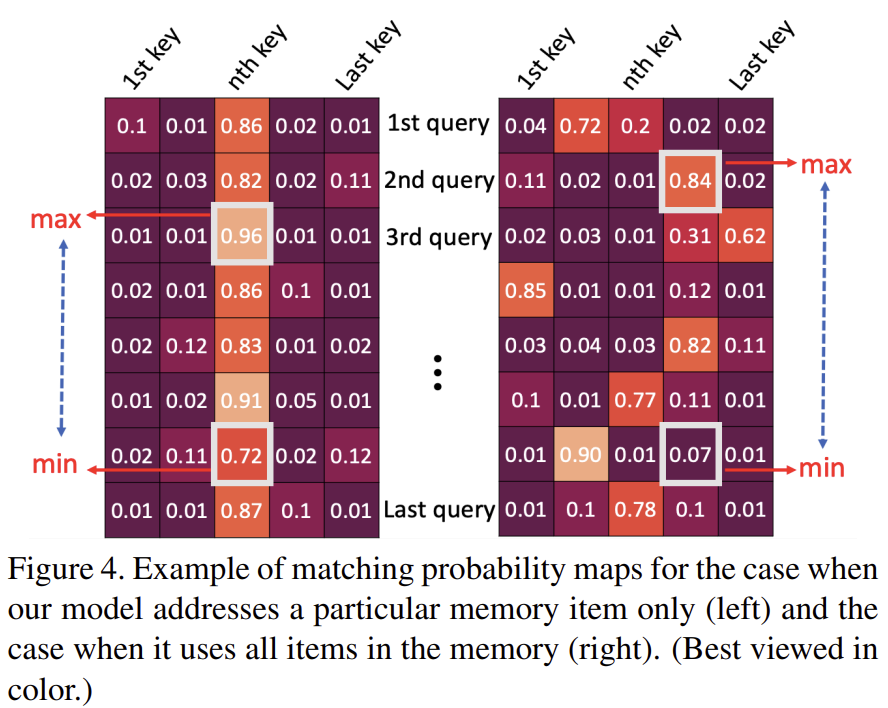
\includegraphics[width=0.85\textwidth]{matching_prob_example.png}
        }{
            \textit{(Matching Probability Example Image Missing)}
        }
    }

    \vspace{0.8em}
    \begin{alertblock}{\small Interpretation}
        \small The SMM accurately detects the moving vehicle blocking the person. It assigns a high matching probability to the distractor region and subtracts those features, allowing the TMM to focus solely on the pedestrian's visible parts across the sequence.
    \end{alertblock}
\end{frame}

% ===== SLIDE: Performance Comparison =====
\begin{frame}{Experimental Results (Our Implementation)}
    \small
    To validate our reproduction of the STMN architecture, we evaluated the trained models on the standard Cumulative Matching Characteristics (CMC) and mean Average Precision (mAP) metrics.
    
    \vspace{1em}
    \begin{table}[]
        \centering
        \renewcommand{\arraystretch}{1.3} % Adds padding to rows
        \begin{tabular}{@{}lcccc@{}}
            \toprule
            \textbf{Dataset} & \textbf{Rank-1 (\%)} & \textbf{Rank-5 (\%)} & \textbf{Rank-20 (\%)} & \textbf{mAP (\%)} \\
            \midrule
            \textbf{MARS} & [FILL]\% & [FILL]\% & [FILL]\% & [FILL]\% \\
            \textbf{iLIDS-VID} & [FILL]\% & [FILL]\% & [FILL]\% & - \\
            \bottomrule
        \end{tabular}
        \caption{Evaluation metrics obtained after training the STMN pipeline.}
    \end{table}

    \vspace{0.5em}
    \begin{block}{\small Key Takeaway}
        \small The high Rank-1 and mAP scores demonstrate that combining Spatial Memory (to remove distractors) and Temporal Memory (to aggregate frames) yields a highly discriminative video representation.
    \end{block}
\end{frame}
